\documentclass{article}
\title{Wave equation simultion} %\LaTeX is a macro for printing the Latex logo
\author{Daniil A. Fadeev}
\newcommand{\dd}{\partial}
\newcommand{\ff}{\frac}
\newcommand{\mathz}{\ooalign{$z$\cr\hfil\rule[.5ex]{.2em}{.06ex}\hfil\cr}}
\newcommand{\vv}{\mathbf}
\newcommand{\chiO}{\chi^{(1)}} 
\newcommand{\chiT}{\chi^{(3)}}
\newcommand{\mum}{\upmu\mathrm{m}}
\newcommand{\ci}{\mathbf{i}}
\newcommand{\op}[1]{\hat{\mathrm{#1}}}
\usepackage{amsmath,esint}
\usepackage[inline]{asymptote}
\usepackage{mathtools} %dcases
\usepackage{upgreek}
\usepackage{hyperref}
\usepackage{graphics}
\usepackage[font=small,labelfont=bf]{caption}

\begin{document}

\maketitle
This is a technical documentation for the physical model and the numerical scheme. This documentation contains derivation of the reduced wave equation, new units to make the model more convenient to work with, finite element scheme, operators approximation and proof-tests to check units, parameters, etc. Ok, let us write our basic equations to start from.






\section{wave equation}
First things first, so meet Maxwell equations:
\begin{eqnarray}
\mathrm{rot} \vv{H} = \ff{1}{c}\ff{\dd \vv{P}}{\dd t}+\ff{4\pi}{c} \vv{j}, \\
\mathrm{rot} \vv{E} = - \ff{1}{c}\ff{\dd \vv{H}}{\dd t}.
\end{eqnarray}
Basic equation for free elextrons current in drude model, compatible with instantaneous (tunneling) ionization:
\begin{equation}
\ff{\dd \vv{j}}{\dd t}=\ff{e^2}{m} n_e \vv{E}.
\end{equation}
And the equation for media bound electrons:
\begin{equation}
\vv{P} = \chiO \vv{E} + \chiT \vv E^3
\end{equation}

From the above equations we have:
\[ \mathrm{rot}\,\mathrm{rot} \vv{E} + \ff{1}{c^2}\ff{\dd^2 \vv P}{\dd t^2}+\ff{4\pi}{c^2}\ff{\dd \vv j}{\dd t}=0 \]
Substituting equation for current and polarzation we obtain wave equation:
\begin{equation}
- \Delta_\perp \vv E -\ff{\dd^2 \vv E}{\dd z^2} + \ff{\chiO - 1}{c^2}\ff{\dd^2 \vv E}{\dd t^2} + \ff{\chiT}{c^2}\ff{\dd^2 \vv E^3}{\dd t^2} +\ff{4\pi e^2}{m c^2} n_e \vv E = 0
\end{equation}
If $rot=0$ we have plasma oscillations:
\begin{equation}
\ff{\dd^2 E}{\dd t^2}+\ff{4\pi e^2}{m} n_e E = 0
\end{equation}
Okay, $4 \pi e^2 n / m$ is a square of plasma frequency. Let us continue.
Passing to new variables:
\begin{eqnarray}
z = z, \\
\tau=t-\frac{z}{c}.
\end{eqnarray}
Using rules
\[ \ff{\dd}{\dd z}=\ff{\dd}{\dd z} -\ff{1}{c}\ff{\dd}{\dd \tau} \]
\[ \ff{\dd}{\dd t}=\ff{\dd}{\dd \tau} \]
We obtain the following equation:
\begin{equation}
\label{eqzt}
\ff{2}{c}\ff{\dd^2 \vv E}{\dd z \dd \tau} - \Delta_\perp \vv E +\ff{\chiO - 1}{c^2}\ff{\dd^2 \vv E}{\dd \tau^2} + \ff{\chiT}{c^2}\ff{\dd^2 \vv E^3}{\dd \tau^2} +\ff{4\pi e^2}{m c^2} n_e \vv E = 0,
\end{equation}
$\dd/\dd z^2$ is neglected here. Plasma density is calculated as follows:
\begin{equation}
n_e = {n_e}_{\mathrm{O}_2} + {n_e}_{\mathrm{N}_2}
\end{equation}
\begin{equation}
\ff{\dd {n_e}_\mathrm{f}}{\dd \tau} = \mathrm{w}_0 (n_\mathrm{f}-{n_e}_\mathrm{f}) A_\mathrm{f} \exp\left(- p_\mathrm{f} \ln\left(\ff{|E|}{E_a}\right) - C_\mathrm{f}\ff{E_a}{|E|} \right)
\end{equation}
here ${}_\mathrm{f}$ subscript stands for ${}_\mathrm{f}$raction, i.e. $\mathrm{f} \in \{ \mathrm{O}_2, \mathrm{N}_2 \}$; $\mathrm{w}_0$ is atomic frequency:
\[ \mathrm{w}_0 = \ff{m e^4} {\hbar^3} = 4.13 \times 10^{16} \, \mathrm{s}^{-1} \]
$n_{\mathrm{O}_2}$ is oxygen neutrals density i.e. $\approx$ 20\% of $n_\mathrm{Air}$, $n_{\mathrm{N}_2}$ is nitrogen neutrals density $\approx$ 80\% of $n_\mathrm{Air}$, $n_\mathrm{Air}=2.7\times 10^{19}\,\mathrm{cm}^{-3}$.

\noindent
$A_\mathrm{f}$, $p_\mathrm{f}$, $C_\mathrm{f}$ were derived in \verb=ioniz_probability_precalc.py= with help of Silaev A.







\section{Dimensionless units:}
We uze:
\[ z_0=\ff{2}{k_0}=0.248\,\mathrm{\mu m}, \ k_0=\ff{2\pi}{\lambda}=80553.65779\,\mathrm{cm}^{-1} \]
\[ \tau_0=\ff{T}{2\pi} = \ff{1}{\omega_0} = \ff{1}{k_0 \, c} = 0.41\,\mathrm{fs}, \ T=\ff{\lambda}{c} \mathrm{\ - \ optic \ period \ at \ 780 \, nm} \]
equation is written as
\begin{equation}
\ff{2}{c \tau_0 z_0}\ff{\dd^2 E}{\dd z \dd \tau} - \ff{1}{x_0^2}\Delta_\perp E + \ff{\chiO-1}{c^2 \tau_0^2} \ff{\dd^2 E}{\dd \tau^2} + \ff{\chiT E_0^2}{c^2 \tau_0^2} \ff{\dd^2 E^3}{\dd \tau^2} + n_0 \ff{4\pi e^2}{m c^2} n_e E = 0,
\end{equation}
where all operators and variables without indexes are dimensionless.
In calculations we use the following form of the equation:
\[ \ff{\dd^2 E}{\dd z \dd \tau} - 2 \Delta_\perp E + \delta n \ff{\dd^2 E}{\dd \tau^2} + K \ff{\dd^2 E^3}{\dd \tau^2} + n_e E = 0. \]
Thus, since $2/(c \tau_0 z_0) = k_0^2$ we have:
\[  \ff{1}{x_0^2}=2 \times \ff{2}{c \tau_0 z_0} = 2 k_0^2 \]
\[ n_0 \ff{4\pi e^2}{m c^2}=k_0^2 \]
\[ \ff{\chiT E_0^2}{c^2 \tau_0^2} = k_0^2 \, K  \]
\[ \chiT = \ff{k_0^2 c^2 \tau_0^2}{E_0^2} K = \ff{1}{E_0^2} K  \]
So
\begin{eqnarray}
x_0=\ff{1}{\sqrt{2}k_0}=0.087\,\mathrm{\mu m} \\
n_0=\ff{\omega^2 m}{4 \pi e^2}=1.8355\times10^{21}\,\mathrm{cm^{-3}}
\end{eqnarray}
In numerical scheme the equation for plasma density reads as follows:
\[ \ff{\dd {n_e}_\mathrm{f}}{\dd \tau} = (n_\mathrm{f}-{n_e}_\mathrm{f}) A_\mathrm{dim} A_\mathrm{f} \exp\left( - p_\mathrm{f} \ln|E| - \ff{C_\mathrm{f}}{|E|} \right) \]
Thus
\[ A_\mathrm{dim} = n_0 \mathrm{w}_0 \left(\ff{n_0}{\tau_0}\right)^{-1} = \mathrm{w}_0 \tau_0 \]
So
\[ A_\mathrm{dim} = \tau_0 \mathrm{w}_0 = 17.1 \]

\noindent
And $E$ has a dimension of atomic field $E_a=5.14220674763\times10^9$ V/cm.
In demensionless units $n_\mathrm{Air}=0.0122$.






\section{SPATIAL OPERATOR}
\subsection{Energy conservation note}
In Fourier space linear part of equation can be written in the form of Shroedinger equation:
\[ \ci\ff{\dd E}{\dd z} + \op A E = 0 \]
Step operator $\op U$ can be found in the following form:
\[ \op U = (1 + \ci \op A dz) (1 - \ci \op A dz)^{-1} \]
Now if $\op U^* = \op U^{-1}$ then obviously energy conserves, i.e. $(\op U E,\op U E) = (E, \op U^* \op U E) = (E, E)$ in corresponding metric.
Let us check if step operator is unitary. First of all $(1 - \ci \op A dz)^{-1}$ can be represented in series in algebraic form since $dz$ is chosen to satisfy Courant's criteria hence series have to converge. So let us do operator conjugation:
\[ \op U^* = (1+\ci \op A^* dz)^{-1}(1-\ci \op A^* dz) \]
We have changed the order since conjugation changes the order of operators $((\op A \op B f , g)=(\op B f , \op A^* g)=(f , \op B^* \op A^* g))$, the inverted operator can be conjugated via Taylor series expansion and then combined back to the form of inverted operator. Now using the same Taylor expansion we can note that $(1 + \ci \op A dz)$ and $(1 - \ci \op A dz)^{-1}$ commute, so $\op U \op U^*$ can be writte in the following form:
\[ \op U \op U^* = (1 - \ci \op A dz)^{-1} (1 + \ci \op A dz) (1+\ci \op A^* dz)^{-1}(1-\ci \op A^* dz) \]
So if $\op A^*=\op A$ then $\op U^* = \op U^{-1}$.
That is quite important to build metric and opertor to preserve that property, and we will do.
\subsection{Approximation}
\begin{figure}[h]
  \centering
\begin{asy}
    include graph;
    defaultpen(fontsize(7pt));
    real R=7.cm;
    pair v = (4.cm,-sqrt(2*4+1)*1cm);
    real ymax = abs(v.y)*1.3;
    draw(circle((0,0),1.cm));
    for(real r=2.cm;r<R;r+=1.cm) {
      if(r<ymax)
        draw(arc((0,0),r,-90-asin(1cm/r)/pi*180,90+asin(1cm/r)/pi*180));
      else
        draw(arc((0,0),r,-asin(ymax/r)/pi*180, asin(ymax/r)/pi*180));
    }
    draw((0,0)--(R+.3,0),EndArrow);
    dot((0,0), red);
    label((0,0),"$f(0)$",N);
    for(real alpha=0;alpha<360;alpha+=90) {
      pair p = rotate(alpha)*(1cm,0);
      dot(rotate(alpha)*(1cm,0), red);
      label(p,"$f(r)$", p/1cm, Fill(white));
    }
    dot((4.cm,0), blue);
    label((4.cm,0),"$f(r_i)$",NE);
    dot((3.cm,0), blue);
    label((3.cm,0),"$f(r_{i-1})$",NE);
    dot((5.cm,0), blue);
    label((5.cm,0),"$f(r_{i+1})$",NE);
    dot((4.cm,sqrt(2*4+1)*1cm), blue);
    label((v.x,-v.y), "$f(r_{i+1})$", NE);
    dot(v, blue);
    label(v, "$f(r_{i+1})$", SE);
    draw((0,0)--v);
    draw(v--(4cm,0), blue);
    label(.5*v, rotate(atan(v.y/v.x)/pi*180)*"$r_i+dr$",NE);
    label((4cm,v.y/2),"$\sqrt{2 r_i \, dr + dr^2}$", E, Fill(white));
\end{asy}
\end{figure}
Laplassian operator can be constructed using 5 points forming cross shape (red for $r_0=0$ and blue for arbitrary node $r_i$). Now let us write operator $\op A$ in three-diagonal form:
\[
\begin{bmatrix}
A_0 & C_0  & \ldots\\
B_1 & A_1 & C_1 & \ldots\\
& & \ddots\\
& \ldots & B_i & A_i & C_i & \ldots\\
& & & & \ddots
\end{bmatrix}
\]
Now (assuming $dr \equiv dx$) and according to drawing, the coefficients can be written in the following form:
\[ B_i = \ff{1}{dx^2} \]
\[ A_i = -\ff{1}{dx^2}\left(2 + \ff{1}{i+1/2}\right) \]
\[ C_i = \begin{dcases}
          \ff{1}{dx^2}\left(2 + \ff{1}{i+1/2}\right),& \text{if } i = 0\\
          \ff{1}{dx^2}\left(1 + \ff{1}{i+1/2}\right),& \text{otherwise}
          \end{dcases}
\]
Let us find if any metric will give $\op A^* = \op A$ with this form of the operator.
Ok lets us assume two vectors $f = \delta(i)$ and $g = \delta(j)$, where
\[ \delta(i) = \{\ooalign{0\cr\raisebox{-2.2ex}{0}},\,0,\,\ldots,\ooalign{1\cr\hfil\raisebox{-2.2ex}{i}\hfil},\ldots,\, 0,\,\ooalign{0\cr\hfil\raisebox{-2.2ex}{n-1}\hfil}\} \]
Now for any $i$ and $j$ we want $(\op A f,g)=(f,\op A g)$, so let us write out these terms:
\[ \op A f = A_i \delta(i) + C_{i-1} \delta(i-1) + B_{i+1} \delta(i+1) \]
\[ \op A g = A_j \delta(j) + C_{j-1} \delta(j-1) + B_{j+1} \delta(j+1) \]
let us use introduce metric as vector $n$, taking into account now
\[ (\op A f, g) = \begin{dcases}
                  A_i n_j,& \text{if }  i=j\\
                  C_{i-1} n_j,& \text{if }  i-1=j\\
                  B_{i+1} n_j,& \text{if }  i+1=j\\
                  0,& \text{else}
                  \end{dcases}
                  = \begin{dcases}
                  A_i n_i,& \text{if }  i=j\\
                  C_{i-1} n_{i-1},& \text{if }  i=j+1\\
                  B_{i+1} n_{i+1},& \text{if }  i=j-1\\
                  0,& \text{else}
                  \end{dcases}
\]
\[ (f, \op A g) = \begin{dcases}
                  A_j n_i,& \text{if }  j=i\\
                  C_{j-1} n_i,& \text{if }  j-1=i\\
                  B_{j+1} n_i,& \text{if }  j+1=i\\
                  0,& \text{else}
                  \end{dcases}
                  = \begin{dcases}
                  A_i n_i,& \text{if }  i=j\\
                  C_{i} n_i,& \text{if }  i=j-1\\
                  B_{i} n_i,& \text{if }  i=j+1\\
                  0,& \text{else}
                  \end{dcases}
\]
Diagonal terms $(i==j)$ brings no problems of course so let us analyse non-diagonal ones. First, both LHS and RHS is non zero only if $i=j+1$ or $i=j-1$; second qualities
\[ C_{i-1} n_{i-1} = B_{i} n_i \]
\[ B_{i+1} n_{i+1} = C_{i} n_i \]
are the same in wide range of $i$ since the second one can be derived from the first; and third: $i\in[1,n-1]$, for the first equality, while for second $i=0$ is fine.
So we are going to use second equality, by skipping $1/dx^2$ we can derive the following:
\[ n_{i+1} = \begin{dcases}
              \left(1+\ff{1}{i+1/2}\right) n_i,& \text{if } i>0 \\
              \left(2+\ff{1}{i+1/2}\right) n_i,& \text{if } i=0
             \end{dcases}
           = \begin{dcases}
              \ff{i+3/2}{i+1/2} n_i,& \text{if } i>0 \\
              4 n_i,& \text{if } i=0
             \end{dcases}
\]
Thus:
\[ n_i = \begin{dcases}
              i+\ff{1}{2},& \text{if } i>0 \\
              \ff{3}{8},& \text{if } i=0
          \end{dcases}
\]
Great, we have a metric that provides conservation of something that approximates energy, since the above expression is something very close to linear dependency on $r$.
\section{DISPERSION}
Dispersion is described with the equation
\[ n-1 = f(\lambda) \]
so we can apply it to our equation since linear part is solved in $\omega$ space.

What is $n$? Basically
\[ |k| = n \omega \]
In wave eqution we use solution in from of
\[ e^{i(\omega t - \mathbf{k} \mathbf{r})} \]
Here with new coordinates $\mathz = z$ $\tau = t - z$ it reads as
\[ e^{i(\omega (\tau+\mathz) - k_z \mathz- \mathbf{k}_\perp \mathbf{r}_\perp)} \]
\[ e^{i(\omega \tau - (k_\parallel-\omega) \mathz- \mathbf{k}_\perp \mathbf{r}_\perp)} \]

In native $\omega, \mathrm{k}$ space the true wave equation reads as
\[ k^2_\parallel + |k_\perp|^2 = n\left(\ff{1}{|\mathrm{k}|}\right)^2 \omega^2 \]

In new coordinates $\mathz, \tau$:
\[ k'_\parallel = k_\parallel - \omega \]
$k_\perp$ and $\omega$ does not change.
Let us use the above relation in  $\omega, \mathrm{k}$ space for true wave equation:
\[ k'^2_\parallel + 2 k'_\parallel \omega + \omega^2 + |k_\perp|^2 = n\left(\ff{1}{|\mathrm{k}|}\right) \omega \]

\[ k'^2_\parallel + 2 k'_\parallel \omega + |k_\perp|^2 = \left(n\left(\ff{1}{|\mathrm{k}|}\right)^2-1\right) \omega^2 \]
In our non-reflective approximation the first term can be neglected ($k'_\parallel \ll \omega$ and even $k'_\parallel \ll |k_\perp|$), so:

\[ 2 k'_\parallel \omega + |k_\perp|^2 = \left(n\left(\ff{1}{|\mathrm{k}|}\right)^2-1\right) \omega^2 \]
\[ |\mathrm{k}| = \left(k'^2_\parallel + \omega^2 - 2 k'_\parallel \omega + |k_\perp|^2\right)^\ff{1}{2}\]

Since in air $n-1 \ll 1$ we will change $k$ to $\omega$ in right hangside and change $n+1$ to $2$:
\[ 2 k'_\parallel \omega + |k_\perp|^2 = 2\left(n\left(\ff{1}{\omega}\right)-1\right) \omega^2 \]

In our dimensionless units it reads as follows:
\[ k'_\parallel \omega + 2 |k_\perp|^2 = 2 \left(n\left(\ff{1}{\omega}\right)-1\right) \omega^2 \]
In air:
\[ n-1=\ff{0.05792105}{238.0185-\lambda^2}+\ff{0.00167917}{57.362-\lambda^2} \]

\section{Electric Field Units and K coefficient}
\subsection{SI, SGS, energy \ldots starting from scratch}
Funny, but I found it usefull to start from very beginning in SI units. The reason for that is that in experiment when you start to deal with power, intensity etc. you always use SI units and it is quite hard to recalculate between SI, SGS and dimensionless. We do not need Maxwell equations we will better start with Coulumb's law:
\[ \mathbf{F}=\frac{q_1 q_2 \mathbf{r}}{4\pi\varepsilon_0 r^3} \]
Ok, we will also use Gauss-Ostrogradsky theorem for the flow:
\[ \oiint_\Sigma \mathbf{E} \mathrm{d} \mathbf{s} = \iiint_V \mathrm{div} \mathbf{E} \, \mathrm{d}^3 r \]
We have to distinguish between electric field strength $\mathrm{div} \mathbf{E}$ and charge density $\rho$. Now if we have a charged area in volume $V$ we can write out electric field in any point $\mathbf{r}$ as follows:
\[ \mathbf{E}(\mathbf{r}) = \iiint_V \frac{\rho(\mathbf{r}') (\mathbf{r}-\mathbf{r}')}{4\pi\varepsilon_0 |\mathbf{r}-\mathbf{r}'|^3} \mathrm{d}^3 r \]
From the above let us calculate $\mathrm{div} \mathbf{E}$:
\[ \mathrm{div} \mathbf{E} (\mathbf{r}) = \iiint_V \frac{\rho(\mathbf{r}')}{4\pi\varepsilon_0 } \mathrm{div}_\mathbf{r}\left(\frac{\mathbf{r}-\mathbf{r}'}{|\mathbf{r}-\mathbf{r}'|^3} \right) \mathrm{d}^3 r' = \iiint_V \frac{\rho(\mathbf{r}')}{4\pi\varepsilon_0 } 4\pi \delta(\mathbf{r}-\mathbf{r}') \mathrm{d}^3 r' = \frac{\rho(\mathbf{r})}{\varepsilon_0} \]
Ofcource we need proper koefficient before Dirac's delta function (if anything $\mathrm{div}(\mathbf{r}/|r|^3)=0$ everywehre except $r=0$ which is clearly seen from direct derivation per coordinate). To get the koefficient before $\delta(\mathbf(r))$ one can write the folowing:
\[ \oiint_\Sigma \frac{\mathbf{r}}{r^3} \mathrm{d} \mathbf{s} = 4 \pi = \iiint_V \mathrm{div}\left(\frac{\mathbf{r}}{r^3}\right) \mathrm{d}^3 \mathbf{r} = \iiint_V k \delta(\mathbf{r}) \mathrm{d}^3 \mathbf{r} = k, \ \text{so} \ k = 4 \pi \]
So
\[ \mathrm{div}\left(\frac{\mathbf{r}}{r^3}\right) = 4\pi \delta(\mathbf{r}) \]
Great, once again the well known equation is written in the following form now:
\[ \mathrm{div} \mathbf{E} (\mathbf{r}) = \frac{\rho(\mathbf{r})}{\varepsilon_0} \]
From now on we can get to the real thing. We need to calculate the energy of electric field and the flux of laser pulse.
We will start from energy. We will calculate energy using a mechanical alternative. Let us start from capacitor:
\begin{center}
\begin{asy}
size(4cm,0);
draw((0,1)--(3,1),linewidth(1pt));
label("$q$", (3,1), (1,1));
draw((0,-1)--(3,-1),linewidth(1pt));
label("$-q$", (3,-1), (1,-1));
for(real x=0.33; x<3-0.33; x+=0.333)
  draw((x,-1)--(x,1), EndArrow);
label("$\mathbf{E}$" ,(0,0), (-1,0));

draw((3,-1)--(3,1), Arrows);
label("$h$", (3,0), (1,0));
label("$S$", (1.5,-1), (0,-1));
\end{asy}
\end{center}

Between plates there is field $E$, now let us very slowly move lower plate to upper one. We are moving slowly to eliminate kinetic enegry from our study. The capacitor is working on our hand and does mechanical work equal to $F h$.
Using Gauss-Ostrograsky therem we can derive that:
\[ E S = \frac{q} {\varepsilon_0} \]
The lower plate is under the action of upper plate so the force acting on lower plate is the field of upper plate which is (according to Gauss-Ostrogradsy theorem):
\[ 2 E_{one} S = \frac{-q} {\varepsilon_0} \]
So from this slow movement of lower plate to upper one we can draw the following amount of energy spent on mechanical work:
\[ h F = h E_{one} q = h \frac{q^2}{2S \varepsilon_0} = \frac{\varepsilon_0}{2} h S E^2 \]
After plates are connected there is no energy left. So the energy density $w_E$ in the beginning of the process was:
\[ w_E = \frac{\varepsilon_0}{2} E^2 \]

Great, let us finally get to EM wave energy. First of all magnetic energy in the EM pulse is equal to electric. The second one factor is that it oscillates, so the energy is half of maximum amplitude. So if maximim aplitude is $E_0$ ($E(z-ct) = E_0 \sin (k_0 (z - ct))$) then energy density is:
\[ w = 2 \frac{\varepsilon_0}{2} E_0^2 \frac{1}{T} \int_T \sin^2(k_0 (z-ct)) \mathrm{d} t = \frac{\varepsilon_0}{2} E_0^2 \]

Now let us consider energy flux $I$ ($W/m^2$) which is $w \cdot c$:
\[ I = \frac{\varepsilon_0 c}{2} E_0^2 \]

The great thing here is that $I$ is measured in $\text W/\text m^2$ and $E_0$ is measured in $\text V/ \text m$ which means that we can use meters or cantimeters with the same coefficient $\varepsilon_0 c / 2$ ($\varepsilon_0 = 8.8541878188(14) \times 10^{-12} \text F / m$, $c=2.99792458 \times 10^8 \text m / \text s$):

\[ E_0 \left[\frac{V}{\text{length unit}}\right] = \sqrt{\frac{2}{\varepsilon_0 c}} \sqrt{I \left[\frac{W}{\text{length unit}^2}\right]} \approx 27.49 \sqrt{I \left[\frac{W}{\text{length unit}^2}\right]} \]

\subsection{Critical power estimation}
Nice! Now we want $P_{cr}$ to be 2.4 GW for our laser pulse with $E$ measured in atomic units $E_a = 5.14220675112(80) \times 10^{11} \text V / \text m$. I think it is easier to work with this type of values than to recalculate $n_2$.
What is critical power? Actually we want to equlize spatial operator action and nonlinearity action.
Let us use Eikonal equation, starting from amplitude-phase representation of $E$:
\[ E = A \exp (\ci \varphi) \]
Now let us do derivatives
\[ \ff{\dd E} {\dd x} = \ff{\dd A}{\dd x} \exp (\ci \varphi) + \ci A \ff{\dd \varphi}{\dd x} \exp (\ci \varphi) \]
\[ \ff{\dd^2 E} {\dd x^2} = \ff{\dd^2 A}{\dd x^2} \exp (\ci \varphi) + 2 \ci \ff{\dd A}{\dd x} \ff{\dd \varphi}{\dd x} \exp (\ci \varphi) - A \left(\ff{\dd \varphi}{\dd x}\right)^2 \exp (\ci \varphi) + \ci A \ff{\dd^2 \varphi}{\dd x^2} \exp (\ci \varphi) \]
\[ \Delta E = \Delta A \exp (\ci \varphi) + 2 \ci (\nabla A \cdot \nabla \varphi) \exp (\ci \varphi) - A |\nabla \varphi|^2 \exp (\ci \varphi) + \ci A \Delta \varphi \exp (\ci \varphi) \]

So real part of quations turns to Eikonal equation:
\begin{equation}
\label{Eikonal}
 - \omega A \ff{\dd \varphi}{\dd z} - 2 \Delta A - 2 A |\nabla \varphi|^2 - \ff{3}{4} \omega^2 K |A|
^2 A = 0
\end{equation}
And imaginary part turns to the equation for envelope:
\[ \omega \ff{\dd A}{\dd z} - 4  (\nabla A \cdot \nabla \varphi) - 2 A \Delta \varphi = 0 \]

Note that
\[ \sin^3\omega t = \ff{3}{4} \sin \omega t - \ff{1}{4} \sin 3\omega t \]

So cosidering flat phase pulse with gaussian transverse shape we can write the following
\[ A = E_0 \exp\left(-\ff{r^2}{r_0^2}\right) \]
\[ \Delta A = E_0 \left(\ff{2 r}{r_0^2}\right)^2 \exp\left(-\ff{r^2}{r_0^2}\right) - E_0 \ff{4}{r_0^2} \exp\left(-\ff{r^2}{r_0^2}\right) = E_0 \ff{4}{r_0^2} \left( \ff{ r^2}{r_0^2}-1\right) \exp\left(-\ff{r^2}{r_0^2}\right) \]
So
\[ E_0 \exp\left(-\ff{r^2}{r_0^2}\right) \ff{\dd \varphi}{\dd z} +  E_0 \ff{8}{r_0^2} \left(1 - \ff{r^2}{r_0^2}\right) \exp\left(-\ff{r^2}{r_0^2}\right) - \ff{3\omega^2 E_0^2K}{4} E_0 \exp\left(-\ff{3 r^2}{r_0^2}\right) = 0 \]
\[ \ff{\dd \varphi}{\dd z} = - \ff{8}{r_0^2} \left(1 - \ff{r^2}{r_0^2}\right) + \ff{3\omega^2 E_0^2K}{4} \exp\left(-\ff{2 r^2}{r_0^2}\right) \approx \ff{3\omega^2 E_0^2K}{4} \left(1-\ff{2 r^2}{r_0^2}\right) - \ff{8}{r_0^2} \left(1 - \ff{r^2}{r_0^2}\right) \]
So it shifts the phase evenly with one rate, while the curvature of the phase shifts with different rate. We need to equlize curvature modification thus the equation:
\[ \ff{3\omega^2 E_0^2K}{4} \ff{2 r^2}{r_0^2} = \ff{8}{r_0^2} \ff{r^2}{r_0^2} \]
\[ \ff{3\omega^2 E_0^2 r_0^2 K}{16} = 1 \]

\[ P = \varepsilon_0 c \oiint \langle E^2 \rangle^T \mathrm{d}^2 \mathbf{r}_\perp = \frac{\varepsilon_0 c E_a^2}{2 k_0^2} \frac{E_0^2}{2} \oiint \exp\left(-2\frac{\mathbf{r}^2_\perp}{r_0^2}\right) \mathrm{d}^2 \mathbf{r}_\perp = \] 
\[ = \frac{\varepsilon_0 c E_a^2}{2 k_0^2} \pi E_0^2 \int \exp\left(-2\frac{\mathbf{r}^2_\perp}{r_0^2}\right) r_\perp \mathrm{d} r_\perp = \]
\[ = \frac{\varepsilon_0 c E_a^2}{2 k_0^2} \frac{\pi E_0^2 r_0^2}{4} \int \exp\left(-2\frac{\mathbf{r}^2_\perp}{r_0^2}\right)  \mathrm{d} \left(2\frac{\mathbf{r}^2_\perp}{r_0^2}\right) = \frac{\varepsilon_0 c E_a^2}{k_0^2} \frac{\pi E_0^2 r_0^2}{8} \]

\[ P_{cr} = \frac{\pi \varepsilon_0 c E_a^2}{k_0^2} \frac{2}{3\omega^2 \mathrm{K}} \]

\[ K = \frac{2 \pi \varepsilon_0 c E_a^2}{3 \omega^2 k_0^2 P_{cr}} \]
For $\lambda=780$ nm, $K\approx 0.00943$.
\subsection{Critical power exact solutions: Townes modes}
Phase curvature on axis gives some approximation for critical power but let us also derive the exact spatial mode that provides perfect compensation of nonlinear and spatial effects. So we are getting back to Eikonal equtions assuming that $\varphi = \alpha z$ (i.e. has no dependency on $r$):
\[ \omega \alpha A  + 2 \Delta A  + \ff{3}{4} \omega^2 K |A|^2 A = 0 \]
This equation can be directly solved by setting some initial $A(r=0)$ and $\alpha$, the above estimations for amplityde and phase velocity can be nice initial values. By fast serching along either $A(r_0)$ or $\alpha$ we can find Townes mode and compare it to previously derived Gaussian beam. I prefer matched on-axis amplitude thus I will serch for proper $\alpha$.

\begin{center}
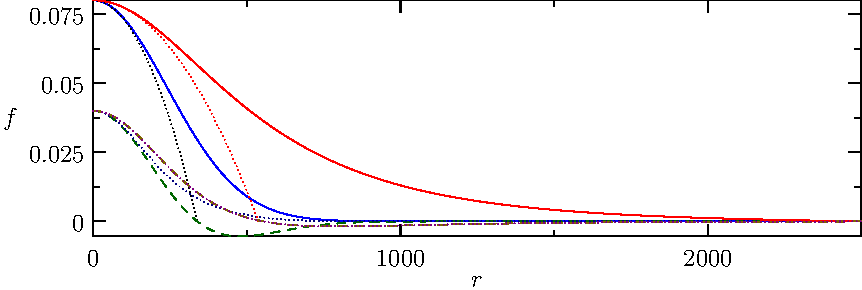
\includegraphics[width=12.3cm]{test/townes/townes.pdf}
\label{figTownes}
\captionof{figure}{Townes and Gaussian modes}
\end{center}

On the plot the blue curve is Gaussian beam plotted according to previous calculations, the red curve is Townes mode. Dotted curves staring from upper left corners of the curves are parabolic curves with curvature correspondig to the accodrding beam profile. To check the solution spatial part $(2 \Delta A)$ and nonlinear plus phase shift part $(\omega \alpha A + 0.75 \cdot \omega^2 K |A|^2 A )$ are plotted with dashed curves and dotted curves. Greenish curves correspond to Guassian, while brownish curves are for Townes and as expected coinsides. Different parablic approxmations with the same on-axis values for Gaussian and Townes are due to different $\alpha$-s for these two bem profiles. Energy ratio betwen that beams is $3.67$ (Townes mode energy is much bigger obviously).

\subsection{Townes mode scaling}
In the above rough Gaussian beam based analysis it was evindent that critical power maintains for different Gaussian beams. Let us show that the shape of Townes mode is the same (with certain scaling of cource) for different on-axis intensities, thus (with linear scaling) critical power will also be a constant indepenednt of on-axis intesity or mode width.
Say we have one Townes solution $A_1(r)$ with sertain $\alpha_1$ now we want another one $A_2(r) = \gamma A_1(\gamma r)$, so let us substitute $A_2(r)$ to Townes euqation:
\[ \omega \alpha \gamma A_1(\gamma r)  + 2 \gamma \Delta_r A_1(\gamma r)  + \ff{3}{4} \gamma^3 \omega^2 K A_1^3(\gamma r) = 0 \]
\[ \omega \alpha \gamma A_1(\gamma r)  + 2 \gamma^3 \Delta_{\gamma r} A_1(\gamma r)  + \ff{3}{4} \gamma^3 \omega^2 K A_1^3(\gamma r) = 0 \]
Let us notate $\gamma r$ as $R$, then:
\[ \omega \alpha \gamma^{-2} A_1(R)  + 2 \Delta_R A_1(R)  + \ff{3}{4} \omega^2 K A_1^3(R) = 0 \]
so $A_2$ can be treated as solution for new $\alpha_2 = \gamma^2 \alpha_1$, i.e. the narrower a solution the bigger is phase velocity. We derived that Townes mode can be rescaled within the same power corresponding to \textit{exact} critical power.

\subsection{Critical power and Kerr coefficient for Townes mode{[Phys. Rev. Lett. 13, 479 (1964)]}}
From the above analysis we know that Townsed mode has $3.67$ greater power than rough gaussian mode from first subsection. So get the same 2.4 GW with townsed we need
\[ K \approx 0.00943 \cdot 3.7 \approx 0.035 \]
\[ \chiT = 1.42 \times 10^{-25} \, \, \, \left[ m^2/V^2 \right] \]
Now we can also calculate coefficients for Kerr and plasma sources in eq (\ref{eqzt})
\[ \dots \ff{\chiT}{c^2}\ff{\dd^2 \vv E^3}{\dd \tau^2} + \ff{4\pi e^2}{m c^2} n_e \vv E \dots \]
\[ \dots \ff{\chiT m}{4\pi e^2 E_0 n_{Air}}\ff{\dd^2 \vv E^3}{\dd \tau^2} + \ff{1}{E_0 n_{Air}} n_e \vv E \dots \]

\section{Kerr coefficient from $n_2$}
Now let us calculate Kerr coefficient from known $n_2$. It is commonly assumed for $n_2 \approx 3 \times 10^{-19} \mathrm{cm}^2/\mathrm{W}$.
Considering (\ref{Eikonal}) for flat wave in out notations we have:

\[ \ff{\dd \varphi}{\dd z} = -\ff{3}{4} \omega K A^2 \]
i.e.
\[ E = A \sin\left(\omega \tau - \ff{3}{4} \omega K A^2 z \right) = A \sin\left(\omega \left( \tau - \ff{3}{4} K A^2 z \right)\right) \]

in real physical quantities it can be rewritten in the following form:

\[ \ff{E}{E_0} = \ff{A}{E_0} \sin\left(\ff{\omega}{\omega_0} \left( \ff{\tau}{\tau_0} - \ff{3}{4} K \ff{A^2}{E^2_0} \ff{z}{z_0} \right)\right) \]
note that $\omega_0 = 2\pi/T = 1/\tau_0 = 2\pi c/\lambda$
\[ E = A \sin\left(\omega \left( \tau - \ff{3}{4} K \ff{A^2}{E^2_0} \ff{z \tau_0}{z_0} \right)\right) = A \sin\left(\omega \left(\tau - \ff{3}{4} K \ff{A^2}{E^2_0} \ff{z}{2 c} \right)\right)\]
Ok now our $\delta n$ is:
\[ \delta n = \ff{3}{8 E_0^2} K A^2 \]
It can be rewritten in terms of intensity:
\[ \delta n = \ff{3}{8 E_0^2} K \cdot 27.49^2 \cdot I \]
So
\[ n_2 = \ff{3}{8 E_0^2} \cdot 27.49^2 \cdot K \]
\[ K = \ff{8 n_2 E_0^2}{27.49^2} = \ff{8 \cdot 3 \cdot 10^{-19} \cdot 5.14^2 \cdot 10^{18}}{27.49^2} = 0.084 \]
\newpage
\section{TESTS}
Below let us do some basic calculations and present the results in \textbf{natural units}. For that basic calculations the results can be derived analytically,
so we can verify each term in wave equation. So once again let us list the eqution and units:
\[ \ff{\dd^2 E}{\dd z \dd \tau} - 2 \Delta_\perp E + \delta n \ff{\dd^2 E}{\dd \tau^2} + K \ff{\dd^2 E^3}{\dd \tau^2} + n_e E = 0. \]
\[ \ff{\dd n_e}{\dd \tau} = \left(\ff{\left|E\right|}{E_0}\right)^{-0.625} \mathrm{exp}\left(-\ff{E_0}{\left|E\right|}\right), \]


\[ z_0=\ff{2}{k_0}=0.248\,\mathrm{\mu m}, \ k0=\ff{2\pi}{\lambda}=80553.65779\,\mathrm{cm}^{-1} \]
\[ \tau_0=\ff{T}{2\pi}=0.41\,\mathrm{fs}, \ T=\ff{\lambda}{c} \mathrm{\ - \ optic \ period \ at \ 780 \, nm} \]
\[ x_0=\ff{1}{\sqrt{2}k_0}=0.087\,\mathrm{\mu m} \]
\[ n_0=\ff{\omega^2 m}{4 \pi e^2}=2\times10^{21}\,\mathrm{cm^{-3}} \]
\[ E_0=5.14220674763\times10^9 \, \mathrm{V}/\mathrm{cm} \]

\noindent
The purpose of those test is not numerical scheme approximation quality check but coefficients, initial conditions and dimenesionless units check.
\newpage
\subsection{VACUUM TEST}
Let us consider a pulse with certain spherical phase front and check whether the focal point will be in appropriate section $z$.
Ok, let input pulse to have the same parabolic phase front for both first and second harmonics:
\[ E|_{z=0} = A_1(\tau + V r_\perp^2) + A_1(\tau + V r_\perp^2) \]
Now let us analyze output from simulation before the first step. Both pulses looks as follows:

\centerline{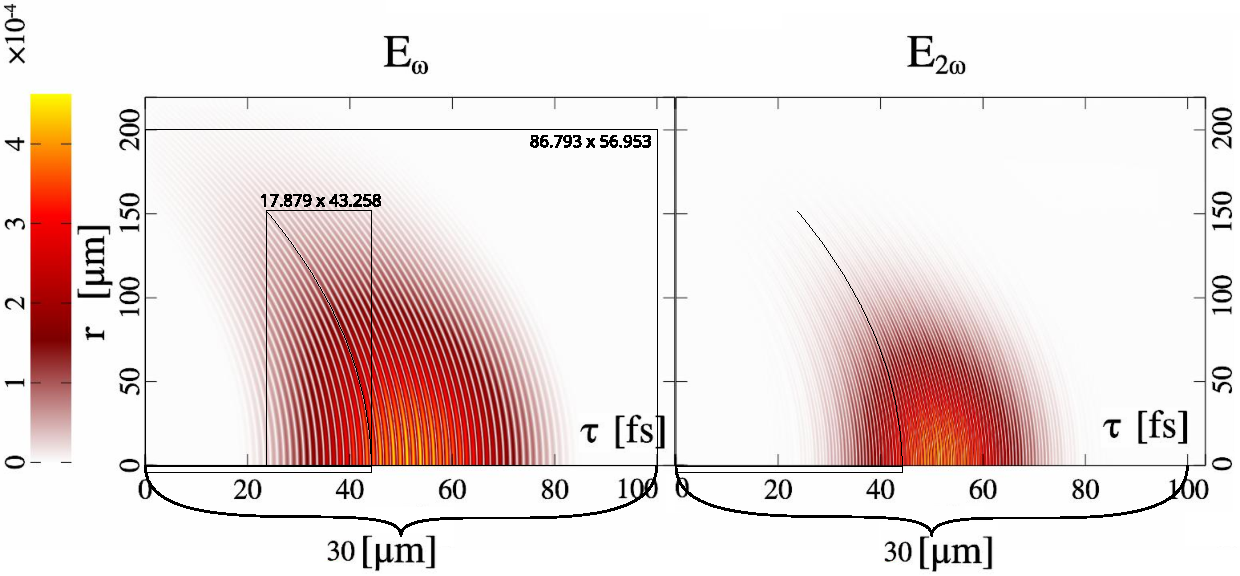
\includegraphics[width=12.3cm]{test/spatial.pdf}}

\noindent
Note that phase fronts for first and second harmonics are the same: note a curved line that follows field extremum.

\noindent
Now let us assume our field is set in $\mathrm{\mathbf{R}}^3$ instead of $\tau, r_\perp$:
\[ E|_{t=0} = A_1\left(z + \ff{r_\perp^2}{z_f}\right) + A_1\left(z + \ff{r_\perp^2}{z_f}\right) \]
Here we assume that
\[ z = z_f - \sqrt{z_f^2-r_\perp^2} \]
where $z_f$ is a focal distance, the above can be represented with Taylor series:
\[ z = z_f - \sqrt{z_f^2-r_\perp^2} \approx \ff{r_\perp^2}{2 z_f} \]
Now using boxes on the drawing we can calculate phase front curvativity:
\[ 30 \mum \cdot \ff{17.879}{86.793} = \ff{1}{2 z_f} \cdot \left(\ff{43.258}{56.953} 200 \mum\right)^2 \]
\[ z_f \approx 1867 \mum\]
So we expect focal distance to be like that. In the above calculation $dz=0.5$ and we dump the field each 333 steps. So the id of focal snapshot shoud be
\[ 1867 \mum / (dz \cdot z0) / 333 \approx 45 \]
Let us take a look at snapshot \#45:

\centerline{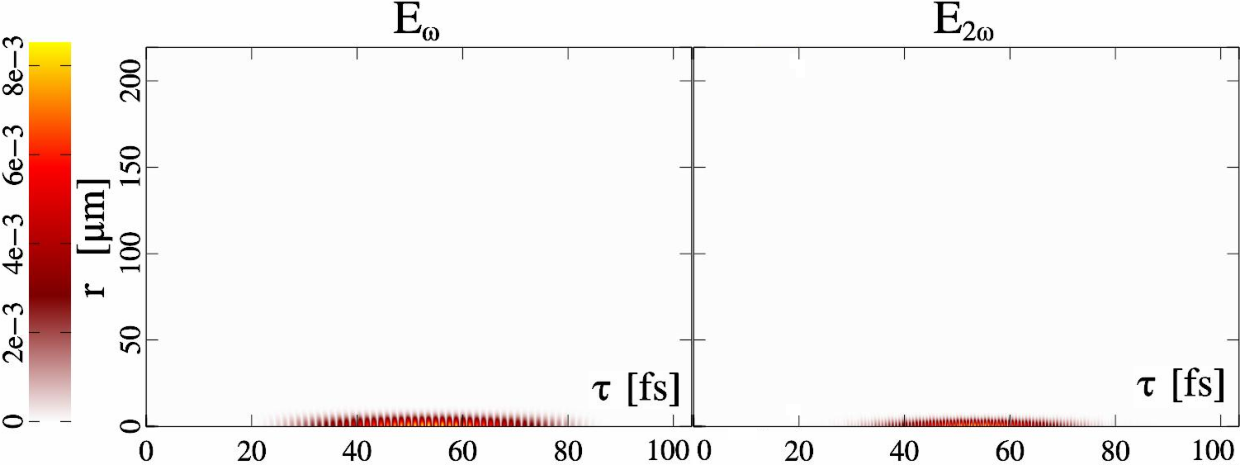
\includegraphics[width=12.3cm]{test/spatial45.pdf}}

\noindent
Ok, we call it a passed test: both first and second harmonics focused at the same correct crossection.

\newpage
\subsection{AIR DISPERSION TEST}
Let us consider a pulse with flat phase and check for phase shift for cases of pulse on $\omega$ and $2\omega$ base frequencies. From \url{refractiveindex.info} for ambient air if follows that:
\[ \delta n = \ff{0.05792105}{238.0185-\lambda[\mum]^{-2}} + \ff{0.00167917}{57.362-\lambda[\mum]^{-2}}  \]
First thing to mention is that on target propagation distances we have almost no change of phase curvature:

\centerline{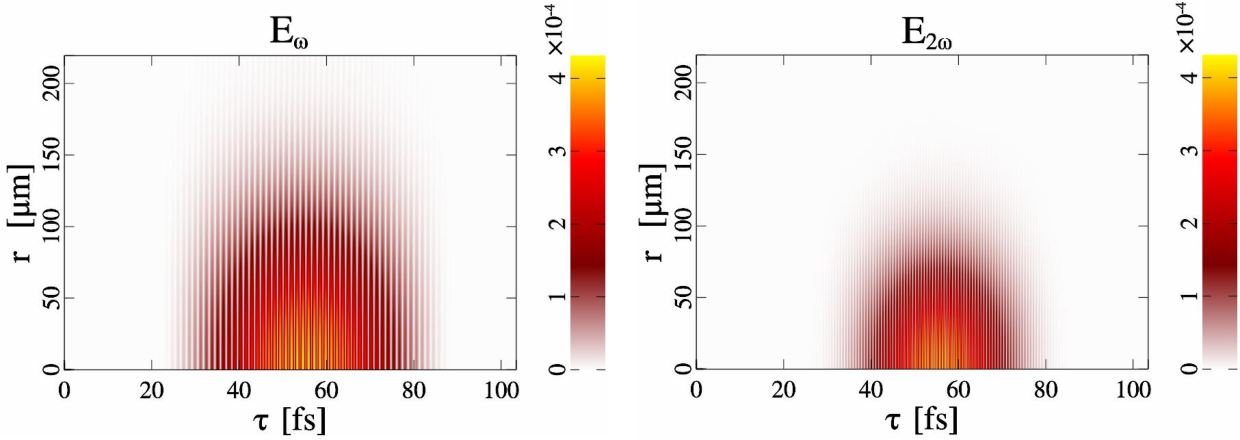
\includegraphics[width=12.3cm]{test/flat_disp_91.pdf}}
The above are field snapshots at the end of propagation. It is clearly seen that phase remains flat.

Zero field somewhere in the center of pulse can be tracked for each crossection z, using hint from previous tracking the continous curve describing phase shift can be obtained. In the picture below red represents base frequency, blue is SG, solid curves are the results without dispersion, dashed curves are from previous calculations with a bug in dispersion law ($\lambda^2$ was used instead of $\lambda^{-2}$), dotted curves ought to be correct ones.

\centerline{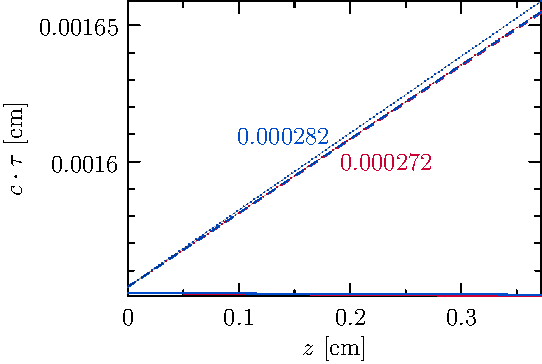
\includegraphics[width=8.3cm]{test/air_disp_test.pdf}}

Slopes are calcualted with residual sum of squares minumization and plotted with thin black solid lines. 
Let us do some basic math, starting from standard form of flat wave:
\[ \mathrm{e}^{\mathrm{i}(\omega t - k z)} \]
In our new coordinates it reads as:
\[ \omega \tau + \ff{\omega}{c} z - k z = 0 \, , \, k = (1+\delta n) \omega / c \]
\[ c \, \tau = \delta n \, z \]
So our slopes ought to be $\delta n$. Using formula for refractive index we get
\[ \delta n_\omega = 0.0002751 \]
\[ \delta n_{2\omega} = 0.0002833 \]
It is quite different from ones on the plot. But the diffs are:
\[ \delta n_{\omega \, sim} - \delta n_\omega = -3.2\times10^{-6} \]
\[ \delta n_{2\omega \, sim} - \delta n_{2\omega} = -1.6\times10^{-6} \]
That diffs are equal to zero dispersion (solid curves). Zero dispersion which appears to be not exaclty zero might be due to intentional changes in dispersion characteristics for stability of solution or it might be numerical dispersion. So we can finally call this a passed test. 

\newpage
\subsection{PLASMA DISPERSION TEST}
Let us consider a pulse with flat phase and check plasma dispersion for cases of pulse on $\omega$ and $2\omega$ base frequencies for two densities of evenly distributed plasma.

\centerline{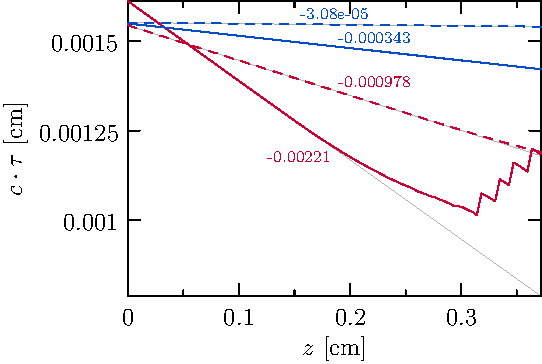
\includegraphics[width=8.3cm]{test/plasma_disp_test.pdf}}
Slopes on the above picture are the result of air dispersion and plasma dispersion. According to previous section the slope corresponds to $\delta n$. Let us compare numerical results $\delta n_\mathrm{sim}$ with theoretical ones for reduced equation $\delta n_\mathrm{red}$ and true one $\delta n_\mathrm{true}$.
Reduced gives : 
\[ \delta n_\mathrm{red} = - \ff{\omega_p^2}{2 \omega^2} \]
true one gives:
\[ \delta n_\mathrm{true} = \sqrt{1 - \ff{\omega_p^2}{\omega^2}} - 1 \]
For numerical we will subtract $\delta n_\mathrm{air}(\omega)$ from previous section.
\begin{center}
\begin{tabular}{ c c c c c }
 density $\times 10^{-18}$ & frequency & $n_\mathrm{sim}$ & $n_\mathrm{red}$ & $n_\mathrm{true}$ \\ 
 4.58 & $\omega_0$ & -0.0012502 & -0.0012500 & -0.00012508 \\ 
 4.58 & $2\omega_0$ & -0.000312545 & -0.00031250 & -0.000311248 \\
 9.17 & $\omega_0$ & -0.00248 & -0.00250 & 0.002503 \\  
 9.17 & $2 \omega_0$ \ & -0.00062515 & -0.0006250 & -0.0006252    
\end{tabular}
\end{center}

It is interesting to note that air dispersion almost cancels out plasma dispersion on SG for quite considerable density of $5\times10^{18}\mathrm{cm}^{-3}$. From the table above it also follows that $\delta n_\mathrm{red}=\delta n_\mathrm{true}$ with quite a good accuracy for densities close to target ones.

\noindent
All in all from the table above we can conclude that plasma dispersion test passed.

\newpage
\subsection{KERR TEST}
Let us consider a pulse with flat phase and find amplitude which provides self-focusing i.e. critical power. 
We are using $K=0.0377$ and together with Townes pulses $\times 0.75$ and $\times 1.25$ variants were analysed:
\begin{center}
\includegraphics[width=13.8cm]{townes_sim/townes_pulses.pdf}
\label{figTownesSim}
\captionof{figure}{a, b -- initial and final $|E_\omega|$ distribution for $.75 \times \mathrm{Townes}(r,\tau)$, c, d -- the same for $\mathrm{Townes}(r,\tau)$, e, f -- the same for $1.25 \times \mathrm{Townes}(r,\tau)$.}
\end{center}
On the pictures it is well seen that Townes pulse remains almost unchnged while weaker one starts to difract and stronger one increases it's onaxis intesity.
It is hard to see any modifications on all three variants except regular monotone changes in amplitude but specrta and THG changes a lot:

\begin{center}
\includegraphics[width=13.8cm]{townes_sim/townes3w_and_spectra.pdf}
\label{figTownesSim_3W_Spec}
\captionof{figure}{a, b -- final $|E_{3\omega}|$ distribution and spectra for $.75 \times \mathrm{Townes}(r,\tau)$, c, d -- the same for $\mathrm{Townes}(r,\tau)$, e, f -- the same for $1.25 \times \mathrm{Townes}(r,\tau)$.}
\end{center}

\noindent
For $1.25 \times \mathrm{Townes}(r,\tau)$ the third harmonic amplitude almost reaches the amplitude of first harmonic.

\newpage
\subsection{BREAKDOWN TEST}
First there are to many coefficients for two fractions ($\mathrm{O}_2$ and $\mathrm{N}_2$) so us just plot theotrtical ionization rates.
\[ \mathrm{w}_{\mathrm{O}_2} = \mathrm{w}_0 \cdot 6.02 \cdot \exp( - 0.123 \cdot \ln F - 0.557 \cdot F^{-1}) \]
\[ \mathrm{w}_{\mathrm{N}_2} = \mathrm{w}_0 \cdot 9.69 \cdot \exp( - 0.868 \cdot \ln F - 0.818 \cdot F^{-1}) \]

\begin{figure}[h]
  \centering
\begin{asy}
import graph;
write("log(2.7)=", log(2.7));
real O2(real F) {
	return 6.018834097463142 * exp( - 0.12307858699746754 * log(F) - 0.5573147246191912 / F);
}
real N2(real F) {
	return 9.691581554890364 * exp( - 0.8679102160158225 * log(F) - 0.8183342643785264 / F);
}

real Air(real F) {
	return 1/17.1 * exp(-0.3125*2 * log(F) - 1.7/F);
}

real pow(real x, real y) {
	return x^y;
}

real Q(int l, int m)
{
	return pow(-1, (m+abs(m))/2)* sqrt((2*l+1)*gamma(l+abs(m)+1)/(2*gamma(l-abs(m)+1)));
}

real w_adk(real B_m, real kappa, real Z_c, real F, int m)
{
	real first_part= pow(B_m,2)/(pow(2, abs(m))*gamma(fabs(m)+1)*pow(kappa,2*Z_c/kappa-1));
	real second_part= pow(2*pow(kappa,3)/F, 2*Z_c/kappa-fabs(m)-1);
	real third_part= exp(-2*pow(kappa,3)/(3*F));
	return first_part*second_part*third_part;
}

real Probab_ioniz_per_time_unit_ADK_N2 (real E_t) 
{
	real Ip=15.58; // first ionization potential for N2 molecule
	real I_H=13.59; // ionization potential for hydrogen atom
  real kappa = sqrt(Ip/I_H);
  int Z_c = 1;
	int m = 0; // magnetic quantum number: for sigma orbitals, m=0; for pi orbitals, m=1
	// From Phys. Rev. A 81, 033423 (2010)
	real C_0_m = 2.68;
	real C_2_m = 1.1;
	real C_4_m = 0.06;
	// From Tong et al., Phys. Rev. A 66, 033402 (2002)
	//real C_0_m = 2.02;
	//real C_2_m = 0.78;
	//real C_4_m = 0.04;
	real B_m = C_0_m*Q(0,m)+C_2_m*Q(2,m)+C_4_m*Q(4,m);
	return 1/3*w_adk(B_m, kappa, Z_c, E_t, m); // 1/3 is due to averaging over the angles, Phys. Rev. A 66, 033402 (2002)
}


real Probab_ioniz_per_time_unit_ADK_O2 (real E_t) 
{
	real Ip=12.06; // first ionization potential for O2 molecule
  real I_H=13.59; // ionization potential for hydrogen atom
  real kappa = sqrt(Ip/I_H);
  int Z_c = 1;
	int m = 1; // magnetic quantum number: for sigma orbitals, m=0; for pi orbitals, m=1
	// From Phys. Rev. A 81, 033423 (2010)
	real C_2_m = 0.52;
	real C_4_m = 0.03;
	// From Tong et al., Phys. Rev. A 66, 033402 (2002)
	//real C_2_m = 0.62;
	//real C_4_m = 0.03;
	real B_m = C_2_m*Q(2,m)+C_4_m*Q(4,m);
	return 2*w_adk(B_m, kappa, Z_c, E_t, m); // 2.0 is due to averaging over the angles, Phys. Rev. A 66, 033402 (2002)	    
}

picture pic;
guide gO2,gN2,gAir;
guide gO2A,gN2A;
scale(pic, Log, Log);

real Fmin = 0.01;
real Fmax = 1.33;
real base = 1.e-64;
for(real F=Fmin; F<Fmax; F+=(Fmax-Fmin)/333) {
	gO2=gO2--(log10(base+F), log10(base+O2(F)));
	gN2=gN2--(log10(base+F), log10(base+N2(F)));
	//gAir=gAir--(log10(base+F), log10(base+Air(F)));
	gO2A=gO2A--(log10(base+F), log10(base+Probab_ioniz_per_time_unit_ADK_O2(F)));
	gN2A=gN2A--(log10(base+F), log10(base+Probab_ioniz_per_time_unit_ADK_N2(F)));
}

draw(pic, gO2,red);
draw(pic, gO2A,red+dashed);
draw(pic, gN2,blue);
draw(pic, gN2A,blue+dashed);
//draw(pic, gAir,gray);
size(pic, 7cm, 4.3cm, point(pic,SW), point(pic,NE));
xaxis(pic, "$\frac{E}{E_a}$", BottomTop, LeftTicks);
yaxis(pic, "$\mathrm{w} \, [\mathrm{w}_0]$", LeftRight, RightTicks);
add(pic.fit());
\end{asy}
\end{figure}
Here dashed curves are plotted using source code provided by Silaev A., solid curves are plotted using above formulae adapted for current numerical algorithm.

\end{document}

